\documentclass{book}
\usepackage[left=2cm, right=2cm, top=2cm, bottom=2cm]{geometry}

\usepackage[spanish]{babel}
\usepackage[utf8]{inputenc}

\usepackage{pdfpages}
\usepackage[pdftex,pdfpagelabels=true]{hyperref} % Para enlaces y metadatos
\usepackage{fontawesome5}
\usepackage{fancyhdr}

\hypersetup{
    colorlinks=true,
    linkcolor=black,  % Color de los enlaces internos (por ejemplo, dentro de la tabla de contenidos)
    urlcolor=magenta,   % Color de los enlaces a URLs
    %%citecolor=green,
    pdfauthor={Moisés Serrano Samudio},
    pdftitle={Villancicos Populares},
    pdfsubject={partituras},
    pdfkeywords={violín,trío,villancicos}
}

\title{Villancicos Populares}
\author{Moisés Serrano Samudio}
\date{24 octubre 2023}

\begin{document}

\newcommand{\CoverName}{Portada}%
\pagestyle{empty}%
\renewcommand{\thepage}{\CoverName}
\includepdf[pages=-]{../extend/0-portada.pdf}

\pagenumbering{roman}


\includepdf[pages=-]{../extend/1-portadilla.pdf}
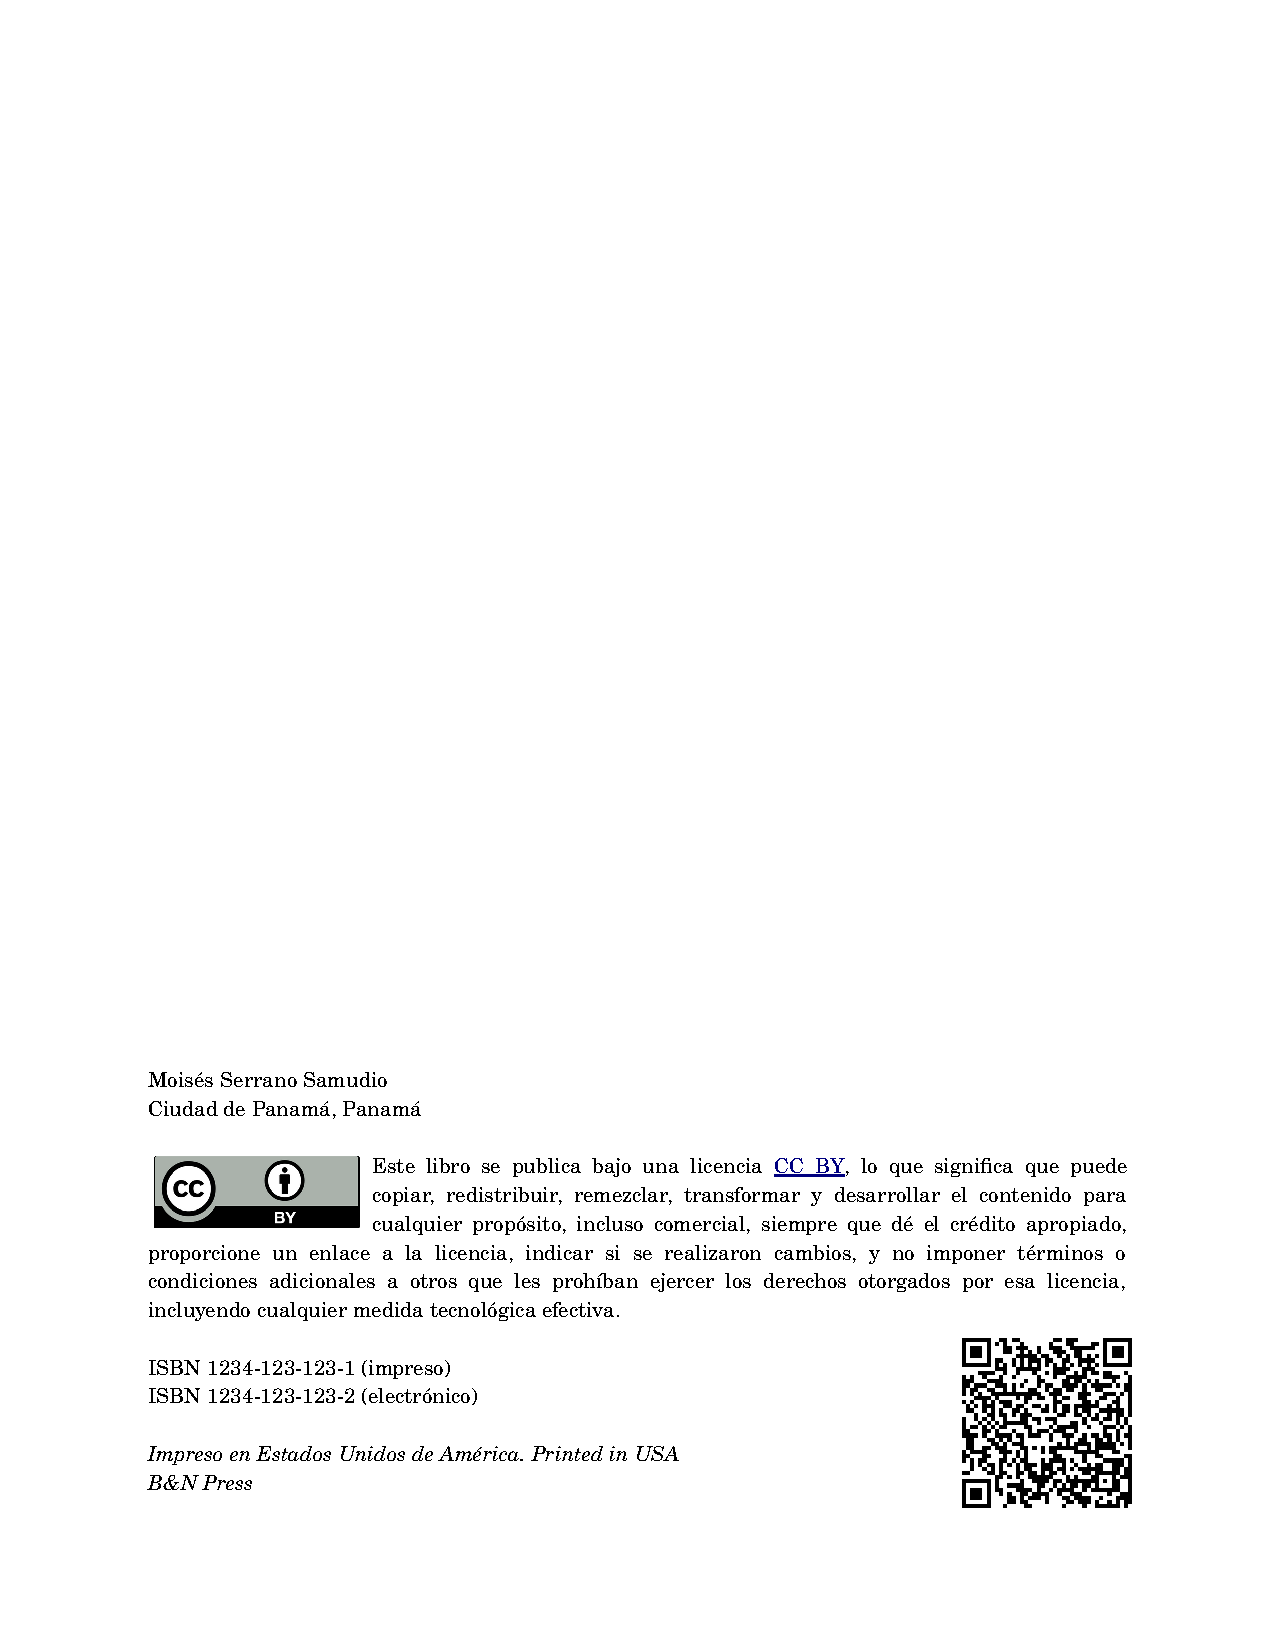
\includepdf[pages=-]{../extend/2-licencia.pdf}
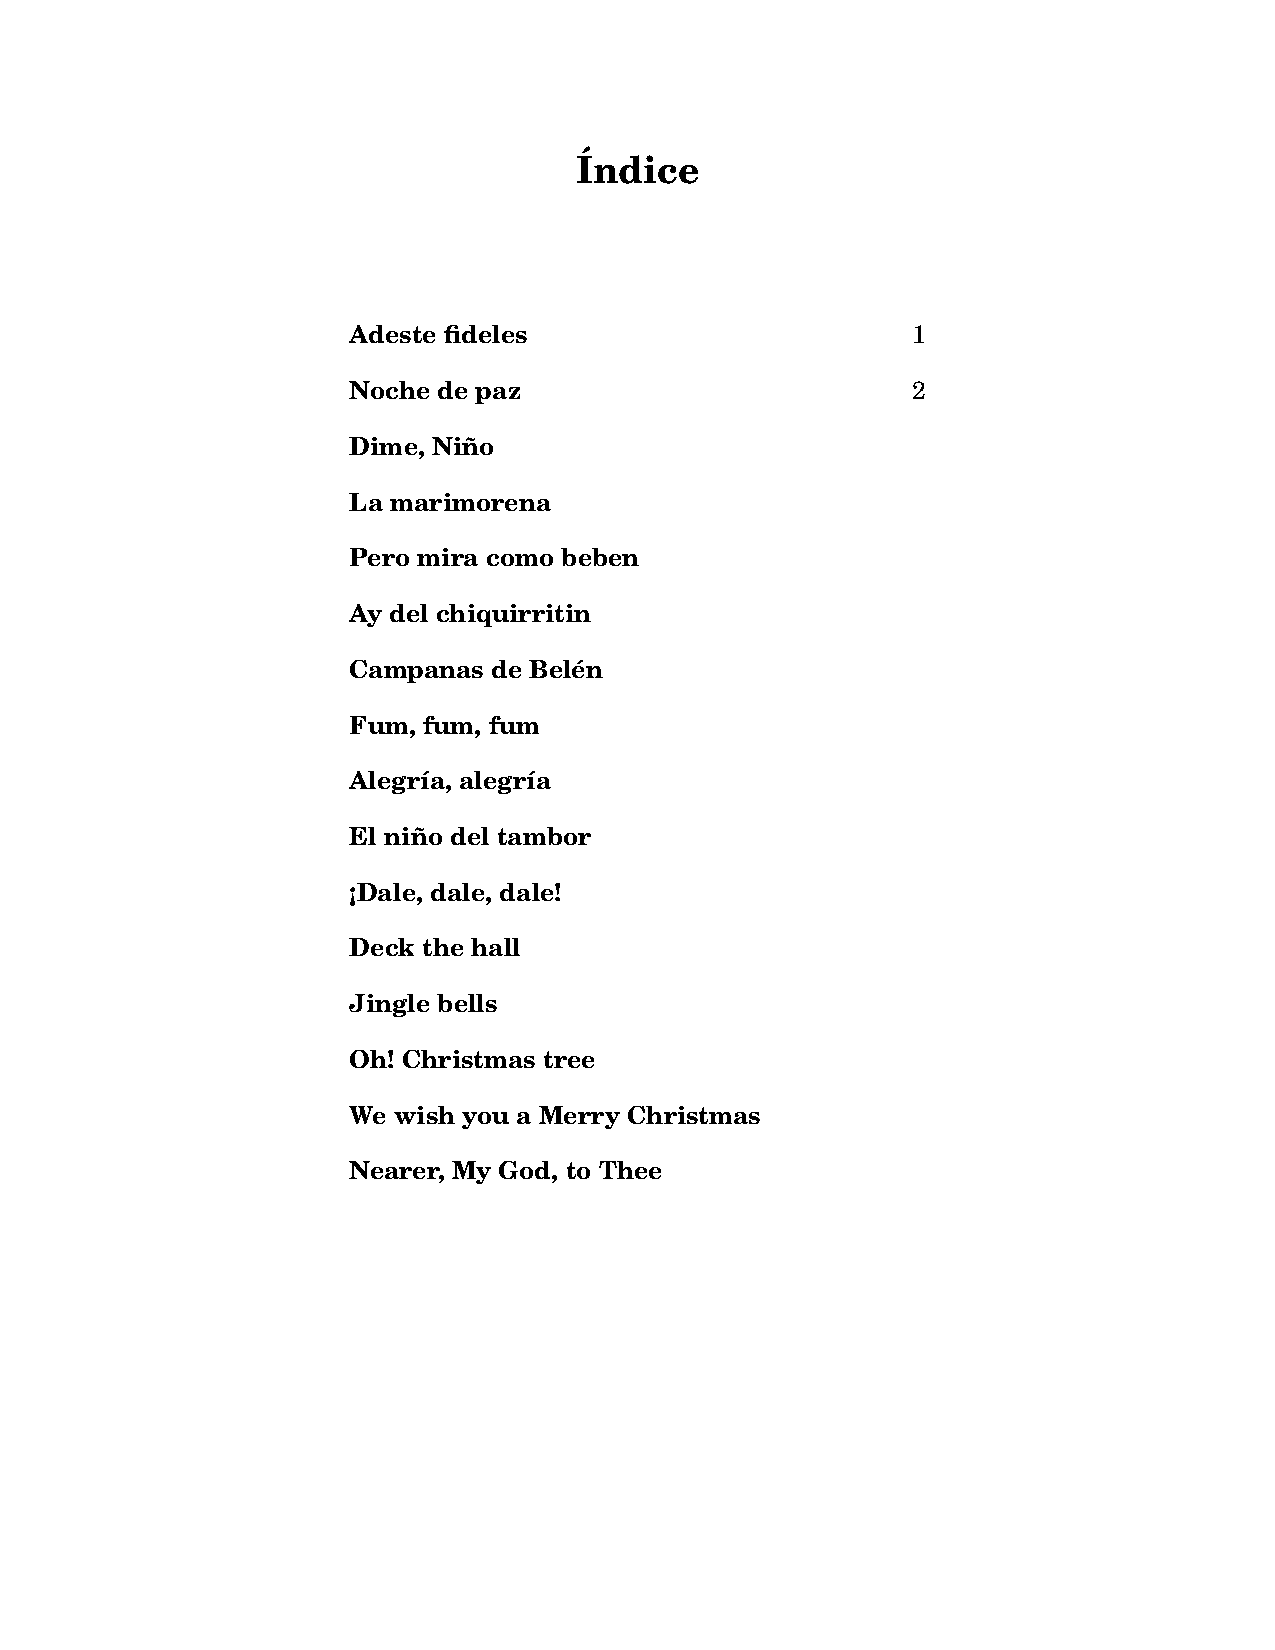
\includepdf[pages=-]{../extend/4-indice.pdf}

\includepdf[pages=-]{../extend/blank.pdf}
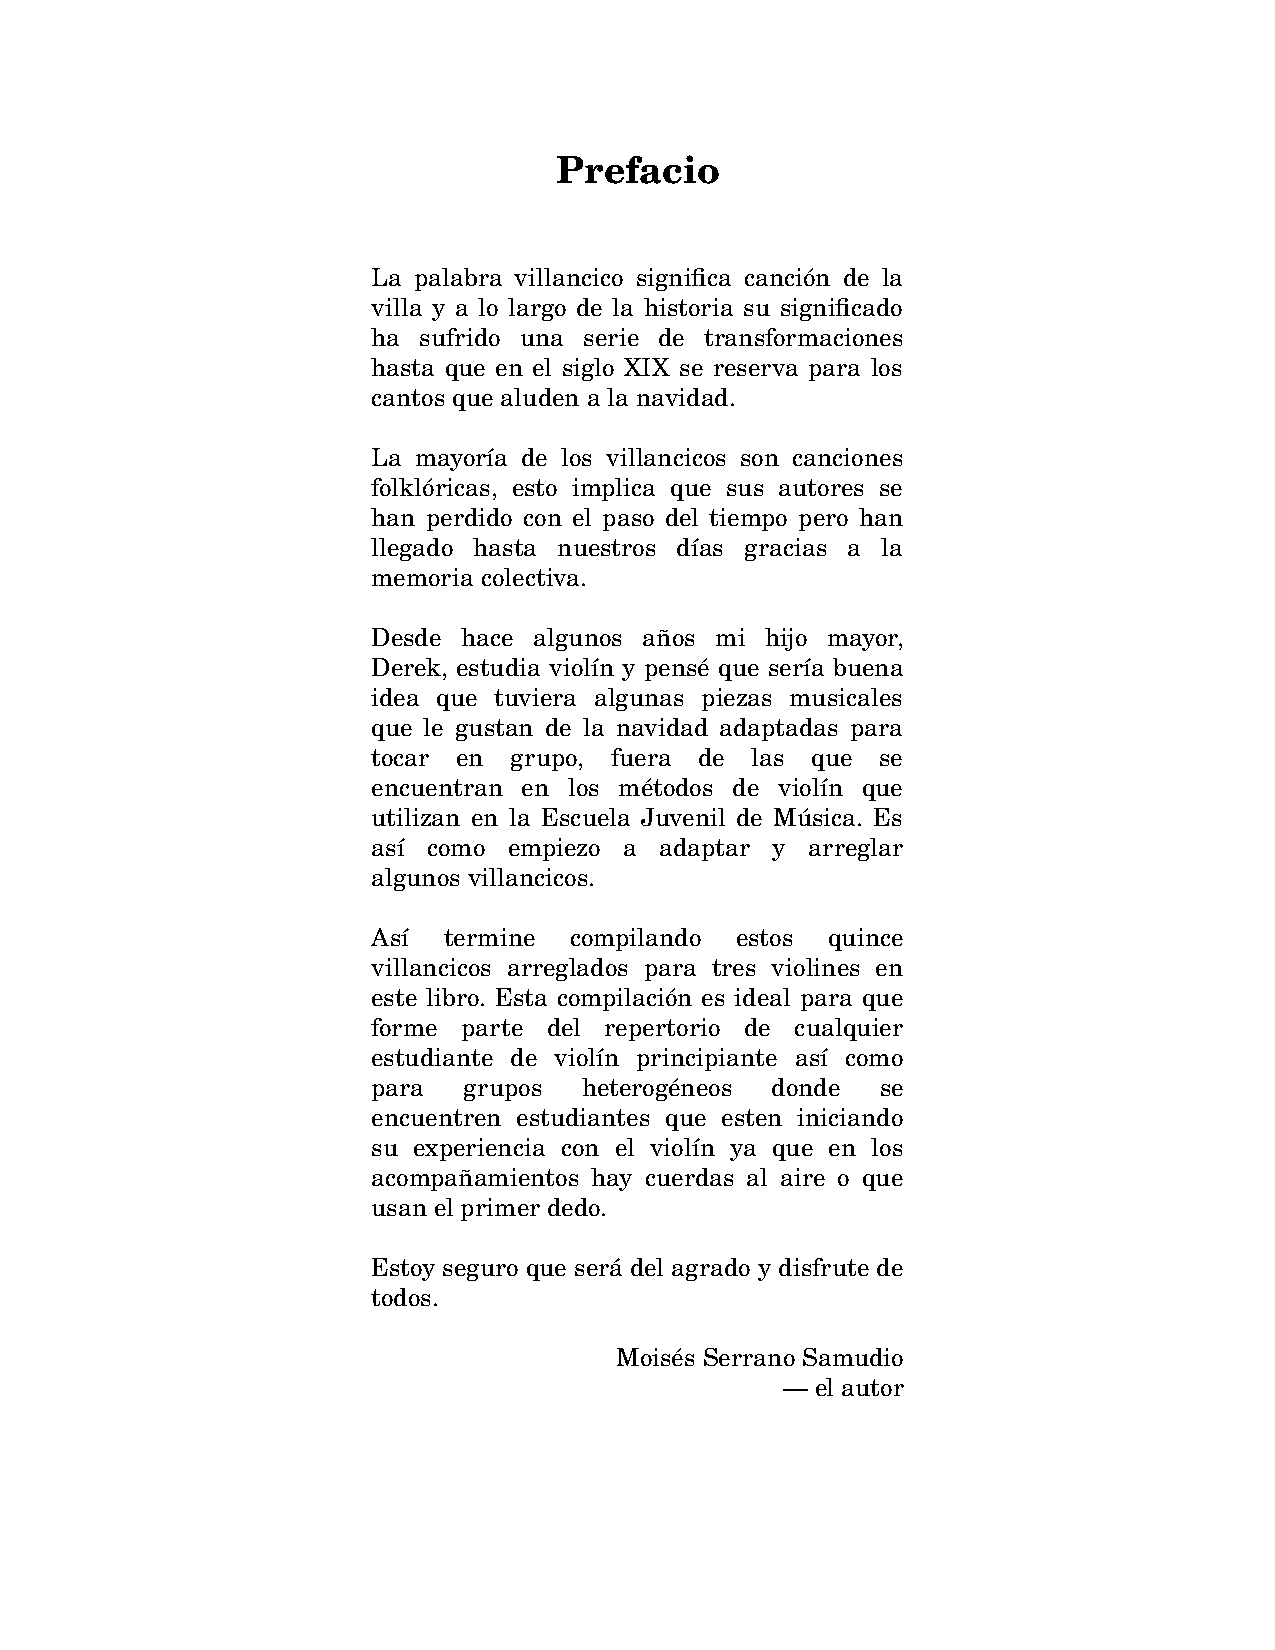
\includepdf[pages=-]{../extend/3-prefacio.pdf}

\includepdf[pages=-]{../extend/blank.pdf}

\pagenumbering{arabic}

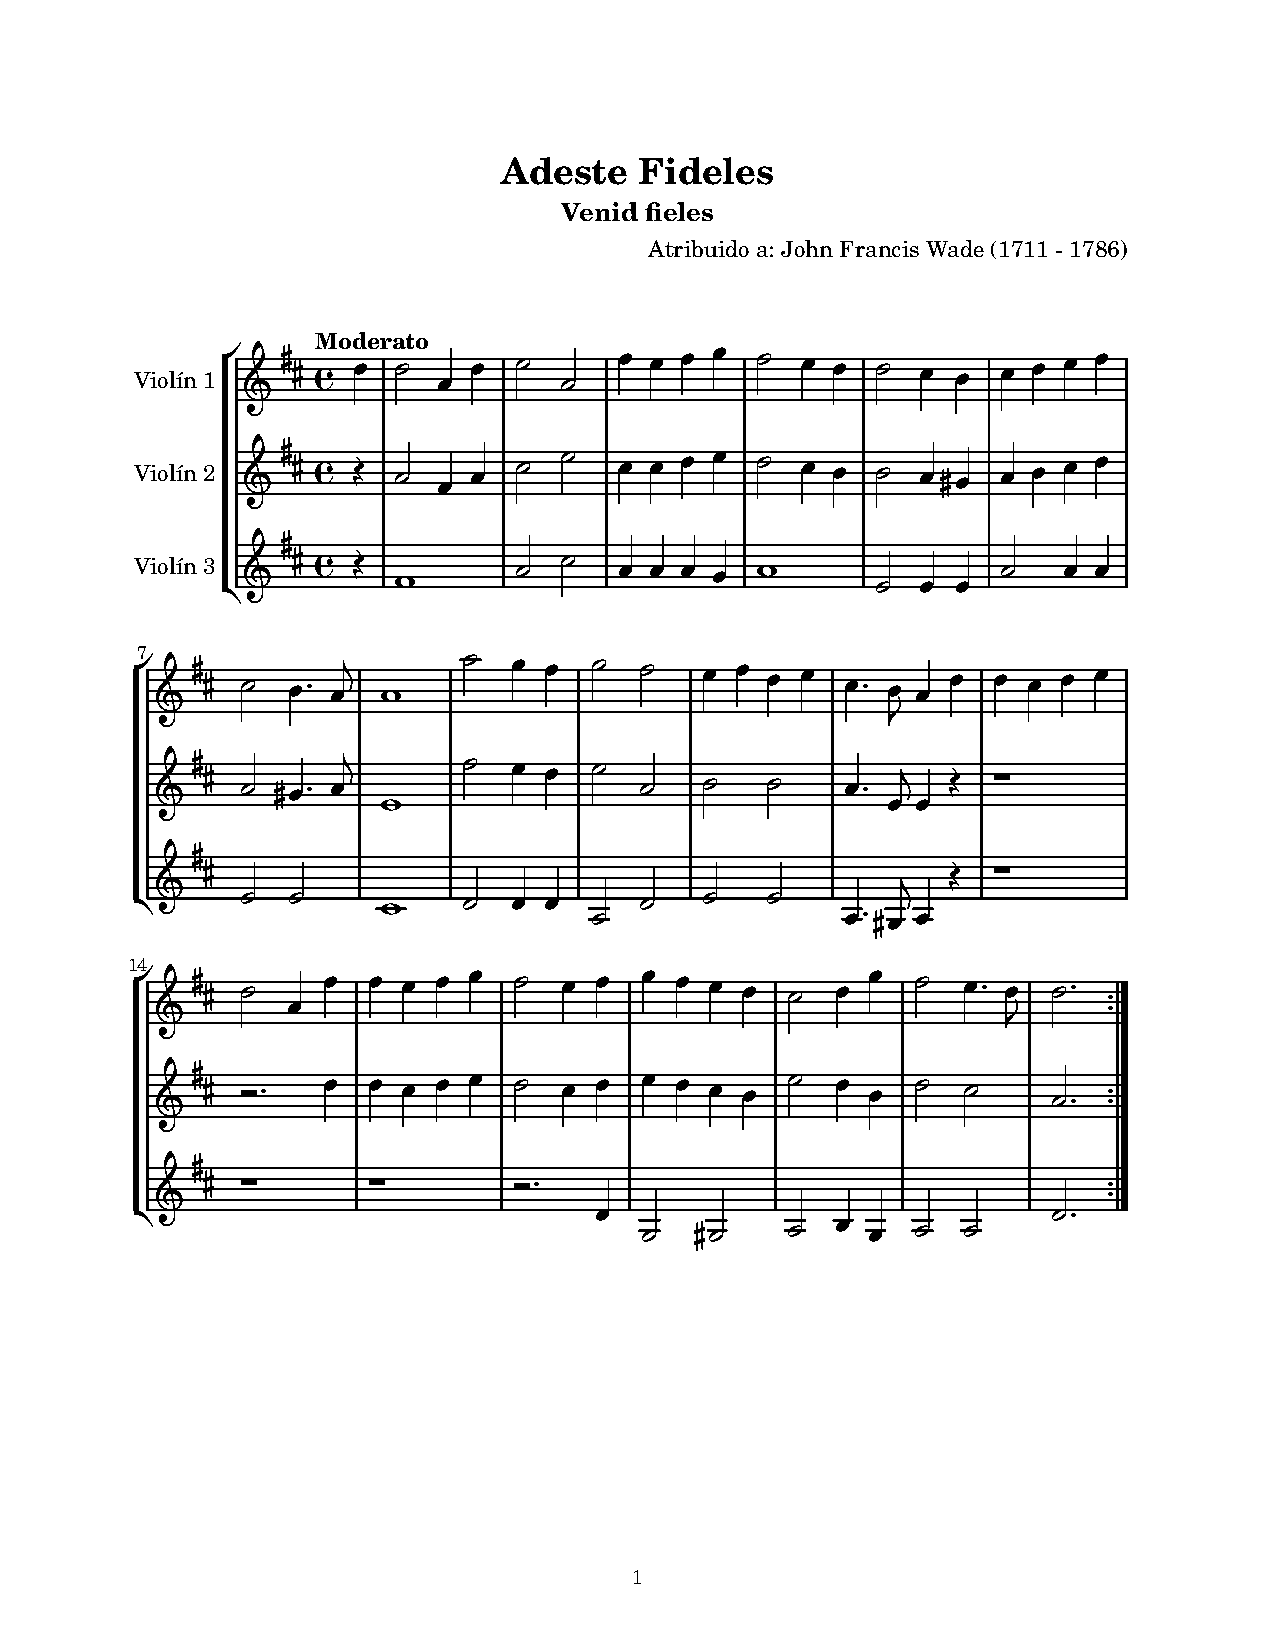
\includepdf[pages=-]{../villancicos.pdf}


\includepdf[pages=-]{../extend/blank.pdf}
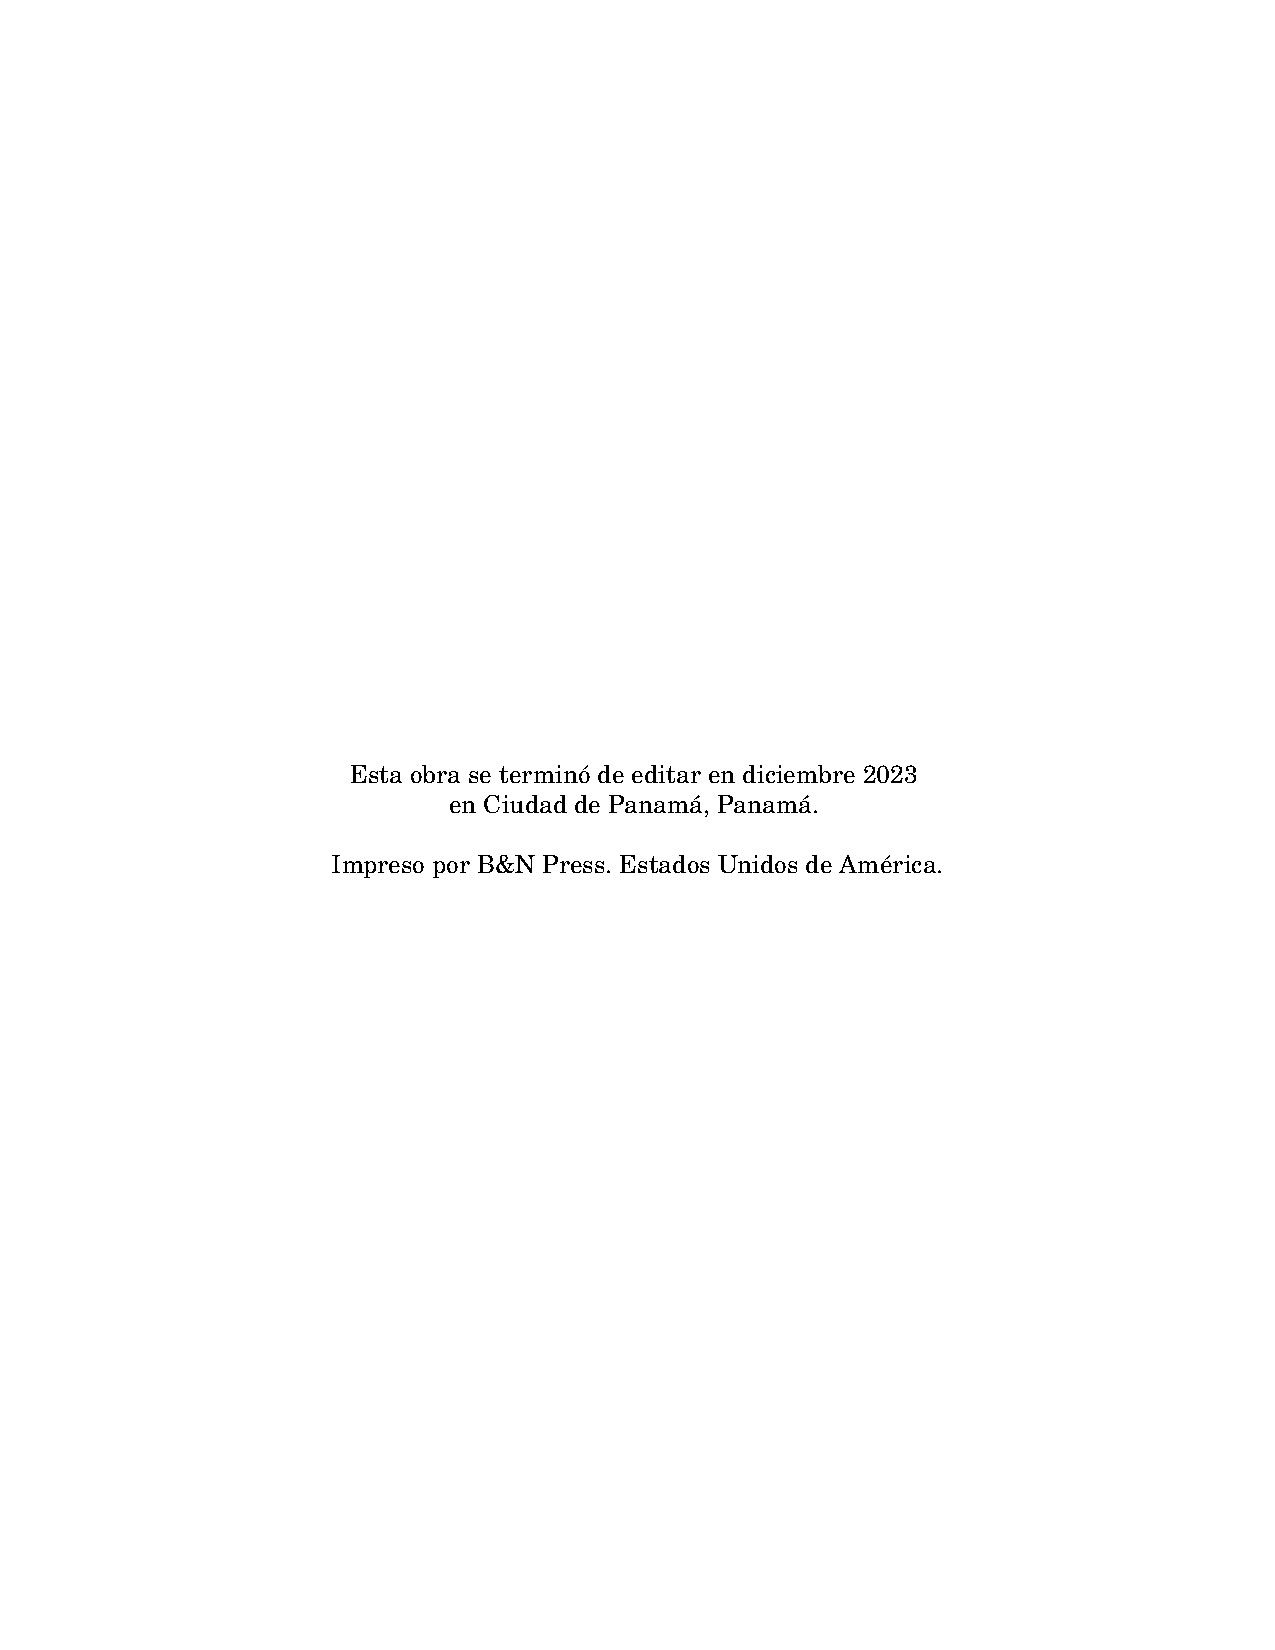
\includepdf[pages=-]{../extend/5-contraportadilla.pdf}

\renewcommand{\CoverName}{Contraportada}%
\pagestyle{empty}%
\renewcommand{\thepage}{\CoverName}
\includepdf{../extend/contraportada.pdf}

\end{document}
